\documentclass[12pt, a4paper]{scrartcl}
\usepackage[ngerman]{babel}
\usepackage{minted}
\title{Coin Counting mit Open CV und Python}
\author{Hoang Son Nguyen}
\date{}
\usepackage{url}
\usepackage{color}
\usepackage{graphicx}
\usepackage{acronym}
\acrodef{hct}[HCT]{Hough-Circle-Transformation}
\graphicspath{ {/.} }
\setlength{\parindent}{0pt}
%\fvset{showspaces}
%\renewcommand\FancyVerbSpace{\textcolor{white}{\char32}}
\begin{document}
\maketitle

\section*{Projekt 2: Geldzähler} 
Auf eine weiße Unterlage fallen Geldmünzen (Euro- und Centstücke in allen Stückelungen). Die Münzen können teilweise übereinander liegen. Der Gesamtbetrag der Münzen ist zu ermitteln.\newline

Erlaubte Tools: OpenCV, Kamera, Standard-Bibliotheken

\section*{Einleitung}
Dieses Projekt wurde mithilfe der Programmiersprache Python umgesetzt. Wir schauen uns erstmal an, wie wir überhaupt ein Bild in unser Programm laden, welches bereits auf unserem Rechner vorhanden ist.\newline

Anschließend, angelehnt an das dritte Praktikum in Bildverarbeitung, werden wir das Projekt mithilfe einer \acl{hct} lösen. Damit lassen sich einfache geometrischen Figuren erkennen. Jedoch statt wie im Praktikum Kanten bzw. Linien zu extrahieren, werden wir diese Methode kennen lernen, die uns Münzumrisse als Kreise aus dem Bild extrahieren kann.\newline

Zum Schluss wenden wir uns noch dem Problem, dass unsere extrahierten Kreisparameter verarbeitet müssen, um den Geldbetrag zu bekommen.

\section{Coin Detection}
Mithilfe der \acl{hct} werden wir die Umrisse unserer Münzen als Kreise erkennen. Dabei speichern wir uns zudem die Parameter um im Anschluss den Geldbetrag ermitteln zu können.

\subsection{\acf{hct}}

Ein Kreis kann in einer zwei-dimensionalen Ebene mit Radius \(r\), Mittelpunkt \((a,b)\)\\ und Kreispunkte \((x,y)\) mit folgender Gleichung beschrieben werden

\[(x-a)^2+(y-b)^2=r^2\]

Die Hough-Transformation wandelt vom Bildraum der \((x,y)\) -Ebene in den Akkumulator- bzw. Hough-Raum der \((a,b)\) -Ebene um. \newline

Den Hough-Raum kann man sich als ein Array bzw. zweidimensionale-Matrix vorstellen. Jeder Pixel unseres Eingangsbildes korrespondiert mit einem zugehörigen Feld und Zähler \emph{counter}. Wir betrachten dazu die Kantenpixel bzw. \emph{edge pixel} aus unserem \emph{preprocessed image}.

Dabei zeichnen wir für ein Kantenpixel einen Kreis mit gewählten Radius \(r\) ein (Abb.1a). Die eingezeichneten Kreispunkte erhöhen den \emph{counter} zu ihrem korrespondierendem Pixel um ein Vote.

\begin{figure}[h]
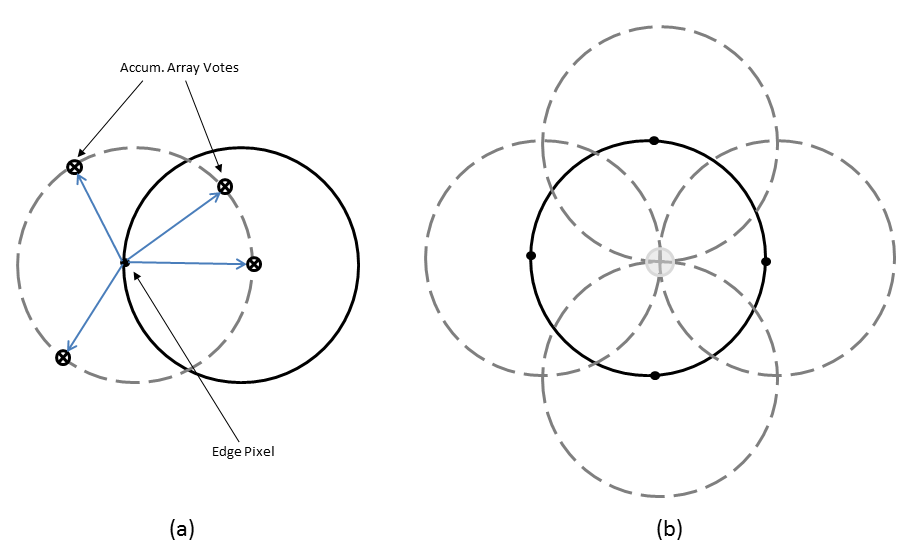
\includegraphics[width=\textwidth]{imfc}
\centering
\caption{\acl{hct} visualisiert}
\end{figure}

Nun wiederholen wir dies für jedes \emph{edge pixel}. Der Hough-Raum quantisiert diese Kreisparameter. Es entstehen dann Punkte mit erhöhtem \emph{counter} dort, wo die Kreispunkte sich überlappen. In Abb.1b beispielhaft für vier \emph{edge pixels} eingezeichnet.\newline

Im Kreismittelpunkt überlappen sich entsprechend die meisten Kreispunkte und es bildet sich ein counter mit Maximum \emph{M}. Damit haben wir unsere Parametrisierung des Kreises mit dem im Mittelpunkt \(M(a,b)\) und zuvor gewählten Radius \(r\) erreicht.\newline

Zu beachten, dass diese Maxima nur entstehen, wenn auch der richtige Radius gewählt wird. Zudem man sich vorstellen kann, dass ein Schwellenwert angeben werden muss, um erhöhte \emph{counter} auszuschließen, die keinen Kreismittelpunkt darstellen.\newline

Man sieht schon, dass die \acl{hct} eine Art „Brute-Force-Ansatz“ zeigt, da man wirklich für alle möglichen Radien \(r\) die \emph{edge pixel} durchlaufen muss. Für eine anschaulichere Darstellung kann man sich an das YouTube Video wenden.

\section{Implementierung}
\subsection{\glqq Image Loading\grqq und \glqq Prepocessing\grqq}
Bevor wir mit unserem Eingangsbild weiter machen, müssen wir dies noch vorverarbeiten. Dieses \emph{preprocessed image} macht es für die anschließende \acl{hct} leichter unsere Münzen zu erkennen. In unserem Fall verwenden wir Gaussian-Blur zur Kontraststeigerung und Canny-Edge zur Kantenbetonung.\newline


\section{Code}

Hier wird noch auf einige Schwierigkeiten hingewiesen, die bei der Erstellung des Codes auftreten könnten.

\begin{minted}
[
frame=leftline,
framesep=2mm,
baselinestretch=1.2,
fontsize=\footnotesize,
%linenos
python3=True
]
{python}
"""
Coin recognition, real life application
task: calculate the value of coins on picture
"""

import cv2
import numpy as np

def detect_coins():
    coins = cv2.imread('./number.jpg', 1)

    gray = cv2.cvtColor(coins, cv2.COLOR_BGR2GRAY)
    img = cv2.medianBlur(gray, 7)
    circles = cv2.HoughCircles(
        img,  # input image
        cv2.HOUGH_GRADIENT,  # type of detection
        dp=1, #inverse ratio of resolution
        minDist = 50, #minimum distance between detected circled
        param1=145, #internal threshold for internal canny edge detector
        param2=60, #threshold for center detection
        minRadius=10,  # mininmum radius to be detected. if unknown, put zero as default
        maxRadius=380,  # max radius to be detected. if unknown, put zero as default
    )

    coins_copy = coins.copy()


    for detected_circle in circles[0]:
        x_coor, y_coor, detected_radius = detected_circle
        coins_detected = cv2.circle(
            coins_copy,
            (int(x_coor), int(y_coor)),
            int(detected_radius),
            (0, 255, 0),
            4,
        )
    print(circles)
    cv2.imwrite("./test_Hough.jpg", coins_detected)

    return circles

def calculate_amount(): #die ratio ist der Quotient bezogen auf den durchmesser 1 cent
    eurparam = {
        "1 cent": {
            "value": 0.01,
            "radius": 16.25,
            "ratio": 16.25/16.25,
            "count": 0,
        },
        "2 cent": {
            "value": 0.02,
            "radius": 18.75,
            "ratio": 18.75/16.25,
            "count": 0,
        },
        "5 cent": {
            "value": 0.05,
            "radius": 21.25,
            "ratio": 21.25/16.25,
            "count": 0,
        },
        "10 cent": {
            "value": 0.10,
            "radius": 19.75,
            "ratio": 19.75/16.25,
            "count": 0,
        },
        "20 cent": {
            "value": 0.20,
            "radius": 22.25,
            "ratio": 22.25/16.25,
            "count": 0,
        },
        "50 cent": {
            "value": 0.50,
            "radius": 24.25,
            "ratio": 24.25/16.25,
            "count": 0,
        },
        "1 Euro": {
            "value": 1,
            "radius": 23.25,
            "ratio": 23.25/16.25,
            "count": 0,
        },
        "2 Euro": {
            "value": 2,
            "radius": 25.5,
            "ratio": 25.5/16.25,
            "count": 0,
        },
    }

    circles = detect_coins()
    radius = []
    coordinates = []

    for detected_circle in circles[0]:
        x_coor, y_coor, detected_radius = detected_circle
        radius.append(detected_radius)
        coordinates.append([x_coor, y_coor])

    smallest = min(radius)
    tolerance = 0.03
    total_amount = 0

    coins_circled = cv2.imread('./test_Hough.jpg', 1)
    font = cv2.FONT_HERSHEY_SIMPLEX

    for coin in circles[0]:
        ratio_to_check = coin[2] / smallest #berechnen aller
        coor_x = coin[0]
        coor_y = coin[1]
        
        for i in eurparam:
            value = eurparam[i]['value']
            ratio = eurparam[i]['ratio']
            #if value == 1:
            #    print(abs(ratio_to_check - eurparam[i]['ratio']))
            #    print(eurparam[i]['value'])

            if abs(ratio_to_check - ratio) <= tolerance:
                print(abs(ratio_to_check - ratio))
                print(value)
                eurparam[i]['count'] += 1 #Zugriff auf Variable
                total_amount += value
                cv2.putText(coins_circled, str(value), (int(coor_x), int(coor_y)), font, 1,
                            (0, 0, 0), 4)

    print(f"The total amount is {total_amount} Euro")
    for i in eurparam:
        pieces = eurparam[i]['count']
        print(f"{i} = {pieces}x")


    cv2.imwrite("./test_Hough.jpg", coins_circled)



if __name__ == "__main__":
    calculate_amount()
\end{minted}
\newpage
\section{Quellen}
\begin{flushleft}
\begin{itemize}
  \item Wikipedia-Artikel zur Hough-Transformation
  \url{https://de.wikipedia.org/wiki/Hough-Transformation}
  \item Anschauliche Darstellung der \acf{hct}
  \url{https://www.youtube.com/watch?v=Ltqt24SQQoI}
  \item Wikipedia-Artikel zu \acl{hct}
  \url{https://en.wikipedia.org/wiki/Circle_Hough_Transform}
  \item Link zur Abbildung 1
  \url{https://de.mathworks.com/help/images/ref/imfindcircles.html}
  \item Artikel zum Erkennen von Kreisem mithilfe \acs{hct}\\
  \url{https://pyimagesearch.com/2014/07/21/detecting-circles-images-using-opencv-hough-circles/}
  \item Methode HoughCircles() OpenCv Documentation
  \url {https://docs.opencv.org/3.4/d4/d70/tutorial_hough_circle.html}
  \item Euromünzen Daten und Abmessungen
  \url {https://de.wikipedia.org/wiki/Eurom%C3%BCnzen}
  \item Coin Detection and Classification using CV-based Strategies
  \url {https://github.com/iambarge/CV-coins-project}
  \item 
  \url {https://dev.to/tinazhouhui/coin-amount-calculation-discovering-opencv-with-python-52gn}
  \item Coin Detection with CZK
  \url {https://github.com/tinazhouhui/computer_vision/blob/master/image_analysis/coin_amount_calculate.py}
  \item detecting circles images using opencv hough circles
  \url {https://pyimagesearch.com/2014/07/21/detecting-circles-images-using-opencv-hough-circles/}
  
\end{itemize}
\end{flushleft}
\end{document}
